%% Copyright 1998 Pepe Kubon
%%
%% `two.tex' --- 2nd chapter for thes-full.tex, thes-short-tex from
%%               the `csthesis' bundle
%%
%% You are allowed to distribute this file together with all files
%% mentioned in READ.ME.
%%
%% You are not allowed to modify its contents.
%%

%%%%%%%%%%%%%%%%%%%%%%%%%%%%%%%%%%%%%%%%%%%%%%%%%
%
%     Chapter 6  
%
%%%%%%%%%%%%%%%%%%%%%%%%%%%%%%%%%%%%%%%%%%%%%%%%

\chapter{Experiments}
\label{ch:exp}

In this chapter, we will evaluate our approach by reporting the experimental results with respect to the running time on computing the subspace skyline on both real data sets and synthetic data sets. We compare the running time of the algorithm with and without using pruning method. Both of the algorithms compute the subspace skyline using \emph{dominating candidate sets} enumerating framework. The only difference between these two algorithms we compare is whether the pruning method is applied.
We implement our algorithms using C++. We use Microsoft Visual Studio 2010 to compile our C++ programs. Experiments were conducted on a PC with an Intel Core(TM) i7-3779 3.40GHz CPU, 16GB main memory and a 900G hard disk, running the Microsoft Windows 7 Enterprise Edition operating system.

\section{Experiments of Skyline Subspace Query on Graph}
\label{ch:exp:graph}
In this section, we will introduce the empirical study on skyline subspace query on graph.
Using the model of Kronecker graph provided by~\cite{leskovec2005realistic}, we generated different sizes of graph.
According to~\cite{leskovec2005realistic}, Kronecker graph has several real world network properties:
heavy tails for the in-degree and out-degree distribution;
heavy tails for the eigenvalues and eigenvectors;
small diameters; and the ``Densification Power Law" (DPL).
We use the MATLAB code from graph500 (\url{http://www.graph500.org/specifications#sec-3_3}) to generate the graph with scale from $15$ to $20$ which corresponds to the number of vertices from $2^{15}$ to $2^{20}$. All the graphs with different sizes are generated from the initial matrix:
\begin{equation}
\begin{bmatrix}
0.3 & 0.24\\ 
0.24 & 0.22
\end{bmatrix}
\end{equation}
with edge factor $2$ which is the expected average degree of the vertices. The label is generated in Pareto distribution which is a Power Law Distribution. We use the Pareto function from a python package numpy to generate the label information of the vertices. We randomly generated 1000 different labels for these graph. Our algorithm run skyline subspace queries in $2$-hops neighbourhood. Figure~\ref{fig:exp:kronecker} shows running time of millisecond per query comparison between the algorithms with and without pruning.

\begin{figure}[h]
    \centering
      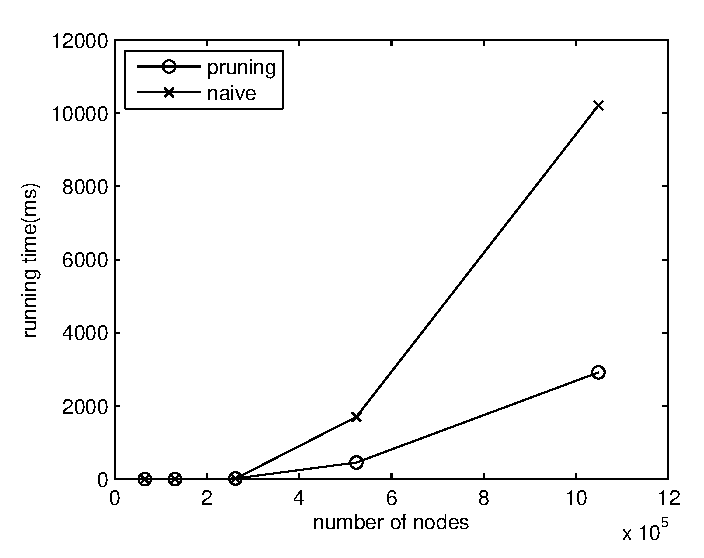
\includegraphics[width=0.7\textwidth]{figs/kronecker}
    \caption{Kronecker graph with 1000 different labels}
    \label{fig:exp:kronecker}
\end{figure}

\begin{table}[h]
    \centering
    \begin{tabular}{|l|l|l|l|}
    \hline
    data sets        & number of nodes & number of edges & number of different labels \\ \hline
    Facebook Network & 4039            & 88234           & 20                         \\ \hline
    DBLP Network     & 906505          & 1656732         & 1000                       \\ \hline
    \end{tabular}
    \label{tab:exp:fb_dblp}
\end{table}

We also do some empirical study on real world datasets. We download a dataset of Facebook network from \emph{Stanford Network Analysis Project} (\url{http://snap.stanford.edu/data/egonets-Facebook.html}). In Figure~\ref{fig:exp:fb}, we show the running time of our program with different numbers of different labels in total. The labels are randomly generated.

\begin{figure}[h]
    \centering
      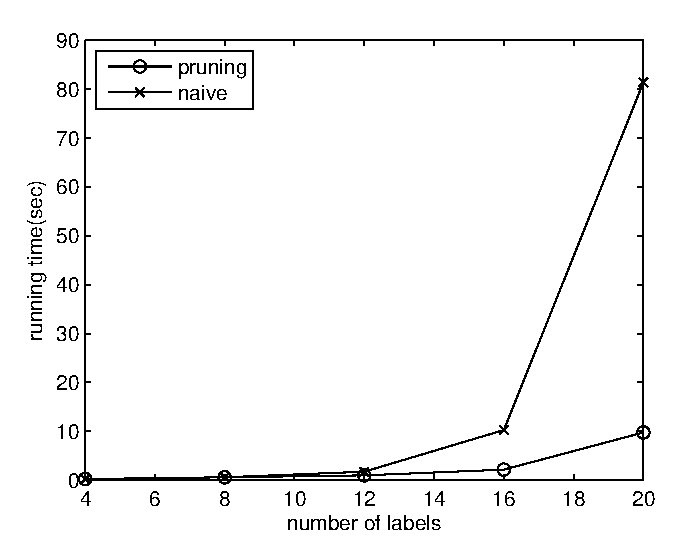
\includegraphics[width=0.7\textwidth]{figs/FB}
    \caption{Facebook network}
    \label{fig:exp:fb}
\end{figure}


We alos use the DBLP dataset from $arnetminer$ (\url{http://arnetminer.org/billboard/citation}) to evaluate the performance of our algorithm. The DBLP dataset provides us the author list of each publication. We build a citation network base these author lists in the following way. We add an edge between author $X$ and author $Y$ if and only if $X$ is one of the top ten co-author of $Y$ and $Y$ is one of the top ten co-author of $X$. We choose the top one thousand most frequent conferences as the labels of the vertices. If an author publishes more than five papers in a conference then we add the corresponding label to that conference to the corresponding label to that vertices. Figure~\ref{fig:exp:dblp} shows the running time of our algorithms on DBLP network.


\begin{figure}[H]
    \centering
      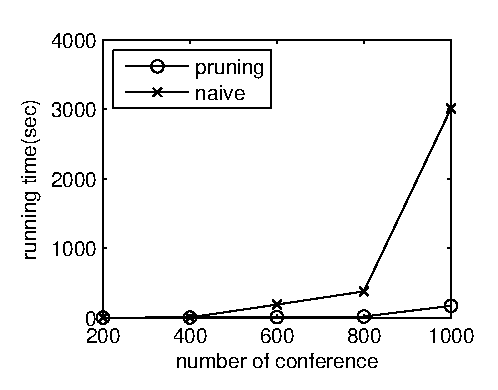
\includegraphics[width=0.7\textwidth]{figs/DBLP}
    \caption{DBLP network}
    \label{fig:exp:dblp}
\end{figure}

\section{Experiments of Spatial Skyline Subspace Query}
\label{ch:exp:spatial}
In this section, we will introduce the empirical study on spatial skyline subspace query. We use the Yelp Academic Dataset (\url{https://www.yelp.ca/academic_dataset}) to evaluate our algorithm. Yelp Academic Dataset provides 13490 different business spot. Each business spot consists of its longitude and latitude information. We use the longitude and latitude information of the business spot as its $XY$ spatial information. The business spot consists of a set of categories information, neighbourhood information and university information. We use those information as the labels of the business spot. Each business spot also contain a stars rating.

In Figure~\ref{fig:exp:yelp20l}, we choose the top 20 most popular categories as the labels of the business spot and we compare the running time of the algorithm with pruning and the algorithm without pruning in the sense of different radius.

\begin{figure}[h]
    \centering
      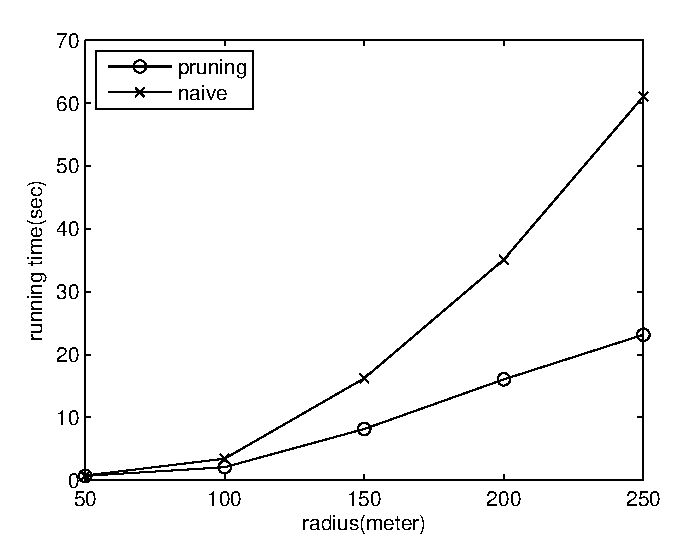
\includegraphics[width=0.7\textwidth]{figs/YelpTop20Labels}
    \caption{Yelp Data Set with Top 20 most popular categories}
    \label{fig:exp:yelp20l}
\end{figure}

In Figure~\ref{fig:exp:yelp300l}, we choose the top $210$ most popular categories as the labels of the business spot. We assign a category to a business spot as a label if the business has the high stars rating among all the business with that category. We also assign the $90$ different neighbourhood information and university information to the business spot as the labels. There is 300 different labels in total. Table~\ref{tab:exp:radius} shows the average number of business spots in different radii in yelp data set.

\begin{figure}[h]
    \centering
      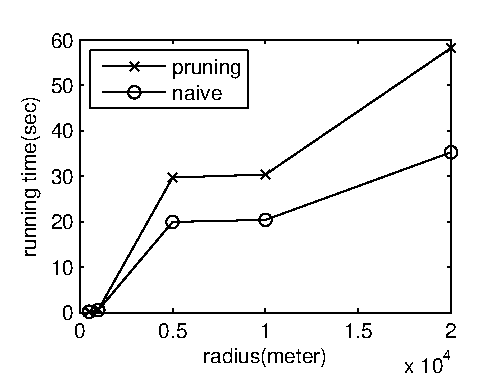
\includegraphics[width=0.7\textwidth]{figs/Yelp300Labels}
    \caption{Yelp Data Set with 300 different labels}
    \label{fig:exp:yelp300l}
\end{figure}


\begin{table}[h]
\centering
\begin{tabular}{|c|c|c|c|c|c|}
\hline
Radius (meters)  & 50  & 100  & 150  & 200   & 250   \\ \hline
Number of Points & 11  & 26   & 42   & 59    & 76    \\ \hline
Radius (meters)  & 500 & 1000 & 5000 & 10000 & 20000 \\ \hline
Number of Points & 159 & 298  & 597  & 657   & 721  \\ \hline
\end{tabular}
\caption{Number of points in certain radii in average.}
\label{tab:exp:radius}
\end{table}

We also evaluate the running times of the algorithm on data with the radius fixed but the number of labels is different. In this experiments, we conduct the empirical study on the large neighbourhood queries whose label collection radius is 10000 meters. we first get a random permutation of the labels. Second, we run the our programs on the first $100$ labels, first $200$ labels, $\dots$, etc. Figure~\ref{fig:exp:yelp10k} shows the running times per query in average.

\begin{figure}[h]
    \centering
      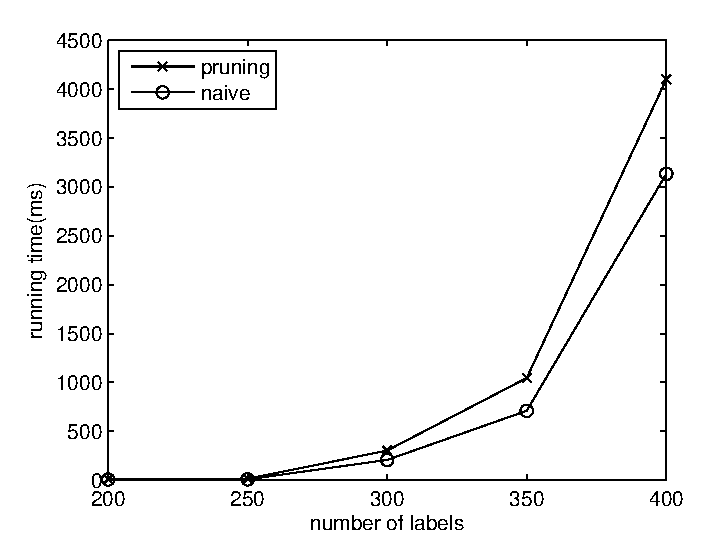
\includegraphics[width=0.7\textwidth]{figs/Yelp10Kmeters}
    \caption{Yelp Data Set in 10000 meters neighbourhood}
    \label{fig:exp:yelp10k}
\end{figure}

Figure~\ref{fig:exp:spatial} shows the running time of spatial synthetic data with 20 different labels. Both the spatial points and the labels of the points are generated randomly in uniform distribution.

\begin{figure}[h]
    \centering
        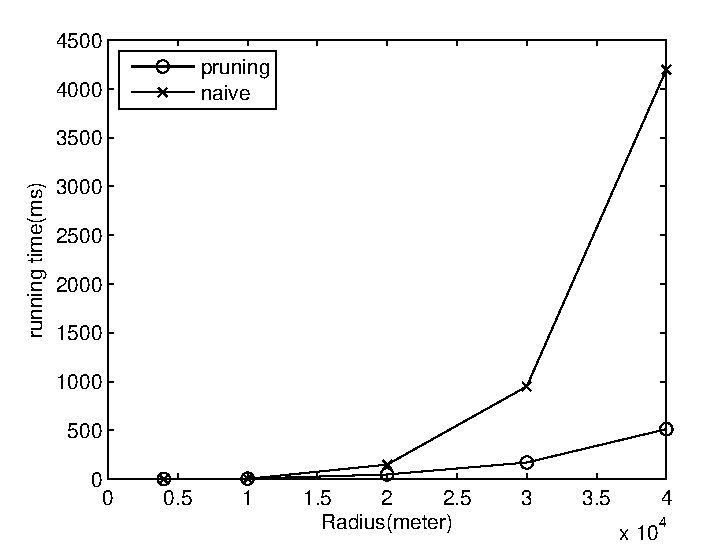
\includegraphics[width=0.7\textwidth]{figs/Spatial}
    \caption{Spatial Synthetic Dataset}
    \label{fig:exp:spatial}
\end{figure}

In summary, the experimental result shows that our algorithm compute the skyline subspace efficiently and the pruning method improve the running time of the programs effectively.